% SPDX-FileCopyrightText: 2022 Severen Redwood <me@severen.dev>
% SPDX-License-Identifier: CC-BY-SA-4.0

\documentclass[headings=standardclasses]{scrartcl}

% SPDX-FileCopyrightText: 2022 Severen Redwood <me@severen.dev>
% SPDX-License-Identifier: CC0-1.0

%% Common Packages and Configuration

%% Layout and Style %%
\usepackage{booktabs}
\usepackage{bookmark}
\usepackage{xcolor}
\usepackage{hyperref}
\hypersetup{
  pdfauthor={Severen Redwood},
  colorlinks=true,
  linkcolor=blue,
  citecolor=blue,
  urlcolor=blue,
}

%% Typography %%
\usepackage{fontspec}
\usepackage{microtype}
\usepackage{siunitx}

%% Maths %%
\usepackage{mathtools}
\usepackage{amssymb}
\usepackage{amsthm}
\usepackage{unicode-math}

% NOTE: cleveref must be loaded here.
\usepackage{cleveref}

% Special sets
% Usual numbers N, Z, Q, R, and C
\newcommand*{\N}{\mathbb{N}}
\newcommand*{\Z}{\mathbb{Z}}
\newcommand*{\Q}{\mathbb{Q}}
\newcommand*{\R}{\mathbb{R}}
\newcommand*{\C}{\mathbb{C}}
% Arbitrary fields
\newcommand*{\F}{\mathbb{F}}
% Circle
\newcommand*{\Si}{\mathbb{S}}
% Torus (n-Torus)
\newcommand*{\T}{\mathbb{}}

% Matrix groups GL and SL
\DeclareMathOperator{\GL}{GL}
\DeclareMathOperator{\SL}{SL}

% Domain, codomain, and image
\DeclareMathOperator{\dom}{dom}
\DeclareMathOperator{\cod}{cod}
\DeclareMathOperator{\im}{im}

% Operations
% Permutations
\newcommand*{\perm}[2]{\prescript{#1}{}P_{#2}}
% Combinations
\newcommand*{\comb}[2]{\prescript{#1}{}C_{#2}}
% Complex conjugate
\newcommand*{\conj}[1]{\overbar{#1}}

% Paired operations
\DeclarePairedDelimiter{\card}{\lvert}{\rvert}
\DeclarePairedDelimiter{\ord}{\lvert}{\rvert}
\DeclarePairedDelimiter{\abs}{\lvert}{\rvert}
\DeclarePairedDelimiter{\norm}{\lVert}{\rVert}
\DeclarePairedDelimiter{\ceil}{\lceil}{\rceil}
\DeclarePairedDelimiter{\floor}{\lfloor}{\rfloor}
\DeclarePairedDelimiter{\cyclic}{\langle}{\rangle}

% Relations
\newcommand*{\divides}{\mathrel{\mid}}
\newcommand*{\notdivides}{\mathrel{\nmid}}
\newcommand*{\subgroup}{<}
\newcommand*{\subgroupeq}{\leq}
\newcommand*{\nsubgroup}{\triangleleft}
\newcommand*{\nsubgroupeq}{\trianglelefteq}

% Binary and hexadecimal numbers
\newcommand*{\bin}[1]{#1_2}
\newcommand*{\hex}[1]{\mathrm{#1}_{16}}

% λ-calculus
\NewDocumentCommand{\labs}{s m m}{
  \IfBooleanTF {#1}
    {(λ#2.\, #3)}
    {λ#2.\, #3}
}
\NewDocumentCommand{\lapp}{s m m}{
  \IfBooleanTF {#1}
    {(#2 \ #3)}
    {#2 \ #3}
}
\NewDocumentCommand{\lshiftt}{m o}{
  \IfNoValueTF {#2}
    {{\uparrow}^{#1}}
    {{\uparrow}^{#1}_{#2}}
}

%% Language %%
\usepackage{csquotes}
\usepackage{polyglossia}
\setdefaultlanguage[variant=newzealand, ordinalmonthday]{english}


\usepackage[style=alphabetic]{biblatex}
\addbibresource{references.bib}

\usepackage{graphicx}
\graphicspath{{figures/}}

\setmainfont{TeX Gyre Pagella}
\setmathfont{TeX Gyre Pagella Math}
\setmathfont{Latin Modern Math}[range=cal]

% Theorem-style Environments
\newtheorem{lemma}{Lemma}
\newtheorem{theorem}{Theorem}
\theoremstyle{definition}
\newtheorem{definition_internal}{Definition}
% Wrapper around definition_internal for adding an "end of definition" symbol.
\newenvironment{definition}
  {\renewcommand{\qedsymbol}{$\triangle$}%
   \pushQED{\qed}\begin{definition_internal}}
  {\popQED\end{definition_internal}}
\newtheorem*{remark}{Remark}
\newtheorem*{note}{Note}
\newtheorem{example}{Example}

\newcommand*{\clam}{\textbf{λ}}

% PDF Metadata
\hypersetup{
  pdftitle={On Representing λ-Terms}
}

\title{On Representing λ-Terms}
\author{Severen Redwood \\ {\small Supervisor: Robert Culling}}
\date{11th February 2023}

\begin{document}

% NOTE: This should be in the preamble, but for some reason it only works
% *within* the document environment...
% I prefer the slanted <= and >= variants.
\let\oldleq=\leq{}
\let\oldgeq=\geq{}
\renewcommand{\leq}{\leqslant}
\renewcommand{\geq}{\geqslant}

\maketitle

\section{Introduction}

The λ-calculus is a formal system of computation based upon function abstraction
and application. First conceived by the American mathematician Alonzo Church in
the 1930s during his research into the foundations of
mathematics~\parencite{church32, church33, church36}, the λ-calculus now
occupies a respectable place at the crossroads of mathematical logic, computer
science, and, perhaps surprisingly, linguistics.

In this report, we describe Church's λ-calculus and its alternate syntactic
representations. The impetus for these topics was the author's work on the
\href{https://turing-tarpit.netlify.app/}{\emph{Turing
Tarpit}}\footnote{https://turing-tarpit.netlify.app/}, an interactive website
that serves as an educational aide for students learning about logic, automata,
and computability. In particular, the topic of alternate syntaxes for the
λ-calculus arose while working on implementing the λ-calculus in a way that
would be reliable and bug free.

\section{Classical λ-calculus}

In this section, we rigorously describe the λ-calculus as envisioned by Church,
which we call the \emph{classical} λ-calculus. Our definitions largely draw from
the text by \textcite{hindley_seldin08}.

\subsection{Syntax}

In order to precisely define any formal system, one must provide two things: a
\emph{syntax}, which determines the form of valid sentences, or expressions, in
the formal system, and a \emph{semantics}, which gives the expressions meaning.
In particular, a semantics is defined \emph{in terms of} a syntax. Thus, if we
wish to define the formal system of computation that is the λ-calculus, we ought
to begin by nailing down its syntax.

\begin{definition}
  Let \(\mathcal{V}\) be a countably infinite set of symbols called
  \textit{variables}.\footnote{
    As a matter of technicality, these symbols must be distinct from the symbols
    \(\lambda\) \(.\) \((\) \()\), which are in use as syntactic delimeters.
  }
  The set of expressions called \textbf{λ-terms} is the smallest set \(\Lambda\)
  such that:
  \begin{enumerate}
    \item If \(v \in \mathcal{V}\), then \(v \in \Lambda\).
    \item
      If \(x \in \mathcal{V}\) and \(t \in \Lambda\), then \(\labs*{x}{t} \in
      \Lambda\), which we call the \emph{abstraction} over \(x\) in \(t\).
    \item
      If \(s, t \in \Lambda\), then \(\lapp*{s}{t} \in \Lambda\), which we call
      the \emph{application} of \(s\) to \(t\). \qedhere
  \end{enumerate}
\end{definition}

Although the above syntax allows for a nearly arbitrary choice of symbols for
variables (by choosing \(\mathcal{V}\)), we shall restrict ourselves to finite
strings of letters from the Latin alphabet, most often only a single letter in
length.\footnote{
  In symbols, if \(\symbb{L} = \{\mathup{a}, \mathup{A}, \mathup{b}, \mathup{B},
  \ldots, \mathup{z}, \mathup{Z}\}\) denotes the set of upper and lowercase
  letters in the Latin alphabet, we let \(\mathcal{V} = \symbb{L}^* = \bigcup_{n
  = 0}^\infty \symbb{L}_n\).
}

\begin{example}
  The following are examples of λ-terms:
  \begin{enumerate}
    \item
      The terms \(x\) and \(y\) are \emph{variables}, as are \(\mathit{id}\) and
      \(\mathit{succ}\) according to our chosen definition of \(\mathcal{V}\).
    \item
      The terms \(\labs*{t}{t}\), \(\labs*{x}{\lapp*{x}{y}}\) and
      \(\labs*{f}{\labs*{x}{\lapp*{f}{x}}}\) are \emph{abstractions}, which
      represent functions.
    \item
      The terms \(\lapp*{s}{t}\) and \(\lapp*{\labs*{x}{x}}{x}\) are
      \emph{applications}, which represent applying a function to an argument.
  \end{enumerate}
\end{example}

As one can see, the syntax of the λ-calculus is quite simple---there are only
three ways to construct a λ-term! And yet, once equipped with a semantics, we
shall obtain a system of computation equivalent in power to a Turing machine, or
indeed any modern programming language, albeit with far fewer syntactic
conveniences.

Before we may define a semantics, however, we require one more thing: the
syntactic notions of \emph{free} and \emph{bound} variables. Such a concept is,
in fact, nothing new; it arises in the usual mathematical notations for
summation, integration, and limits. For example, in the integral
\[ \int_0^\pi \sin(\alpha{}x)\,\mathup{d}x, \]
the variable \(x\) in \(\sin(\alpha{}x)\) is \emph{bound} by \(\mathup{d}x\),
while the variable \(\alpha\) remains unbound, i.e.
\emph{free}.\footnote{
  In integral calculus, it is not uncommon to see \emph{dummy variable} used to
  refer to a variable bound by an integral.
}
Consequently, the variable \(x\) is, in effect, unimportant---the value of the
expression depends only on \(\alpha\). Similarly, in the λ-term
\[ \labs*{f}{\lapp*{f}{x}}, \]
the variable \(f\) in \(\lapp*{f}{x}\) is bound by \(\lambda{}f.\), while the
variable \(x\) is free.

To make this notion rigorous, we state the following
definition:

\begin{definition}
  Let \(\symbf{FV} : \Lambda \to \mathcal{P}(\mathcal{V})\) and \(\symbf{BV} :
  \Lambda \to \mathcal{P}(\mathcal{V})\) be functions such that, for all \(x \in
  \mathcal{V}\) and \(s, t \in \Lambda\),
  \begin{enumerate}
    \item
      \(\symbf{FV}(x) \coloneqq \{x\}\) and
      \(\symbf{BV}(x) \coloneqq \varnothing\);
    \item
      \(\symbf{FV}(\labs{x}{t}) \coloneqq \symbf{FV}(t) \smallsetminus \{x\}\)
      and \(\symbf{BV}(\labs{x}{t}) \coloneqq \symbf{BV}(t) \cup \{x\}\);
    \item
      \(\symbf{FV}(\lapp{s}{t}) \coloneqq \symbf{FV}(s) \cup \symbf{FV}(t)\) and
      \(\symbf{BV}(\lapp{s}{t}) \coloneqq \symbf{BV}(s) \cup \symbf{BV}(t)\).
  \end{enumerate}
  When \(x \in \symbf{FV}(t)\), we say that \(x\) is \textbf{free} in \(t\).
  Likewise, when \(x \in \symbf{BV}(t)\), we say that \(x\) is \textbf{bound} in
  \(t\).
\end{definition}

Be aware that the notions of free and bound variable are \emph{not} mutually
exclusive---it is entirely possible that a variable in a term is both free
\emph{and} bound. For example, the variable \(x\) is both free and bound in the
term \(\lapp{\labs*{x}{\lapp{f}{x}}}{x}\) as \(x\) is bound in the left subterm,
but free in the right subterm. Although such terms are permitted by the syntax,
they are in practice discouraged due to causing possible confusion.

\subsection{Semantics}

As it stands, the λ-calculus is currently inert; we have a rigorously defined
way to \emph{construct} λ-terms, but no way of performing \emph{computation}
with these terms. By considering an abstraction \(\labs*{x}{t}\) to represent a
function given by a well-defined rule \(t\), and an application
\(\lapp*{\labs*{x}{t}}{s}\) to represent the application of this function to an
argument \(s\), we wish to define a way in which this application is carried
out.

So, let us look at how we compute with functions in ordinary mathematics.
Suppose \(f : \Z \to \Z\) is a polynomial function defined by
\[ f(n) = n^2 + n + 1. \]
Then, we denote the application of \(f\) to the number \(2\) by \(f(2)\) and
compute the result by systematically replacing each \(n\) to obtain the result
\[ f(2) = 2^2 + 2 + 1 = 7. \]
The crucial procedure in this example is the act of replacing \(n\), the
variable bound by the function, in the rule \(n^2 + n + 1\) that defines \(f\)
by the argument \(2\). Such a procedure is called \emph{substitution} and forms
the core operation of the λ-calculus.

\begin{definition}
  Given a variable \(x \in \mathcal{V}\) and a term \(s \in \Lambda\), let \([x
  \mapsto s] : \Lambda \to \Lambda\) be a function such that, for all \(y \in
  \mathcal{V}\) and \(t_1, t_2 \in \Lambda\),
  \begin{enumerate}
    \item \([x \mapsto s]y \coloneqq s\) if \(x = y\);
    \item \([x \mapsto s]y \coloneqq y\) if \(x \neq y\);
    \item \([x \mapsto s]\labs*{y}{t_1} \coloneqq \labs*{y}{t_1}\) if \(x = y\);
    \item
      \([x \mapsto s]\labs*{y}{t_1} \coloneqq \labs*{y}{[x \mapsto s]t_1}\) if
      \(x \neq y\) and \(y \not\in \symbf{FV}(s)\);
    \item
      \([x \mapsto s]\labs*{y}{t_1} \coloneqq \labs*{z}{[x \mapsto s][y \mapsto
      y]t_1}\) if \(x \neq y\) and \(y \in \symbf{FV}(s)\), where \(z\) is
      chosen such that \(z \not\in \mathbf{FV}(s) \cup \mathbf{FV}(u)\);
    \item
      \([x \mapsto s]\lapp*{t_1}{t_2} \coloneqq \lapp*{[x \mapsto s]t_1}{[x
      \mapsto s]t_2}\). \qedhere
  \end{enumerate}
\end{definition}

While substitution is relatively straightforward for variables and applications,
special care must be taken when working with abstractions. In particular,
clauses 4 and 5 are specifically formulated to avoid what is called
\emph{variable capture}. For example, naively replacing \(y\) with
\(\labs*{f}{\lapp*{f}{x}}\) in the body of \(\labs*{x}{\lapp*{x}{y}}\) results
in the term \(\labs*{x}{\lapp*{x}{\labs*{f}{\lapp*{f}{x}}}}\). However, the free
occurrence of \(x\) in \(\labs*{f}{\lapp*{f}{x}}\) has now become \emph{bound}
by the outermost abstraction, and so we say that the variable has been
\emph{captured}.

To resolve this issue, we simply rename the clashing bound variable since,
ultimately, its name does not matter. Thus, we might rename the bound variable
\(x\) to \(z\) in \(\labs*{x}{\lapp*{x}{y}}\) before substitution to obtain the
result \(\labs*{z}{\lapp*{z}{\labs*{f}{\lapp*{f}{x}}}}\). In the terminology of
the λ-calculus, we call such renaming of bound variables \emph{α-conversion}.

\begin{example}~
  \begin{enumerate}
    \item \([x \mapsto y]x = y\), but \([x \mapsto y]x = x\).
    \item
      \([f \mapsto \lapp*{g}{t}]\labs*{x}{\lapp*{f}{x}} =
      \labs*{x}{\lapp*{\lapp*{g}{t}}{x}}\), but
      \([f \mapsto \lapp*{g}{t}]\labs*{f}{\lapp*{f}{x}} =
      \labs*{f}{\lapp*{f}{x}}\).
    \item
      \([y \mapsto \labs*{f}{\lapp*{f}{x}}]\labs*{x}{\lapp*{x}{y}} =
      \labs*{z}{\lapp*{z}{\labs*{f}{\lapp*{f}{x}}}}\) (note the necessary
      α-conversion).
  \end{enumerate}
\end{example}

Using our robust definition of substitution, we now state the rule that
defines how computation is performed within the λ-calculus.

\begin{definition}
  For \(x \in \mathcal{V}\) and \(s, t \in \Lambda\), a term of the form
  \[ \lapp*{\labs*{x}{t}}{s} \]
  is called a \textbf{β-reducible expression}, or \textbf{β-redex} for short.

  Let \(\rightarrow_\beta\) be a binary relation on \(\Lambda\) called
  \textbf{β-reduction} such that
  \[ \lapp*{\labs*{x}{t}}{s} \rightarrow_\beta [x \mapsto s]t \]
  and \(n \rightarrow_\beta n\) for any other term \(n\) which is \emph{not} a
  β-redex.
\end{definition}

% With β-reduction defined, we now have a definition of what function, or
% \emph{abstraction}, application means in the λ-calculus.

\begin{example}~
  \begin{enumerate}
    \item \(\lapp*{\labs*{x}{x}}{y} \rightarrow_\beta y\).
    \item
      \(\lapp*{\labs*{f}{\lapp*{f}{x}}}{\lapp*{g}{t}} \rightarrow_\beta
      \lapp*{\lapp*{g}{t}}{x}\).
    \item
      \(\lapp*{\labs*{f}{\labs*{x}{\lapp*{f}{x}}}}{x} \rightarrow_\beta
      \labs*{y}{\lapp*{x}{y}}\) (note the necessary α-conversion).
  \end{enumerate}
\end{example}

\section{Alternate Representations}

While the symbolic names of the classical λ-calculus work well for human
understanding, the potential for variable capture complicates the operation of
substitution and is known to introduce subtle bugs in computer implementations
if one is not careful. To address this issue, researchers and practitioners have
introduced a variety of alternate syntaxes for the λ-calculus, of which we
present the most common.

\subsection{The Barendregt Convention}

Our first \enquote{alternate syntax}, named after the Dutch logician Henk
Barendregt, is merely a convention. The idea is simple: ensure that all names
bound by abstractions are both mutually distinct and separate from any names
used for free variables. For example, the term
\(\lapp*{\labs*{a}{\labs*{b}{\lapp*{a}{b}}}}{b}\) violates the Barendregt
convention since \(b\) is both the name of a bound variable in the left subterm
and also the name of a free variable in the right subterm. By contrast, the term
\(\lapp*{\labs*{a}{\labs*{b}{\lapp*{a}{b}}}}{c}\) does \emph{not} violate this
convention.

Under the Barendregt convention, it is impossible for variable capture to arise
since, for any term, the set of free variables and the set of bound variables
are disjoint. Thus, supposing the convention is \emph{consistently} adhered to,
the defining rules for substitution reduce to the following:
\begin{enumerate}
  \item \([x \mapsto s]y = s\) if \(x = y\);
  \item \([x \mapsto s]y = y\) if \(x \neq y\);
  \item \([x \mapsto s]\labs*{y}{t_1} = \labs*{y}{t_1}\) if \(x = y\);
  \item
    \([x \mapsto s]\labs*{y}{t_1} = \labs*{y}{[x \mapsto s]t_1}\) if \(x \neq
    y\);
  \item
    \([x \mapsto s]\lapp*{t_1}{t_2} = \lapp*{[x \mapsto s]t_1}{[x \mapsto
    s]t_2}\). \qedhere
\end{enumerate}

Unfortunately, while effective for ridding worries of variable capture in simple
terms, the Barendregt convention becomes easy to accidentally violate when
working in more complicated contexts.

\subsection{Nameless Terms}

Another, perhaps surprising, way of easing the pains associated with symbolic
names is to simply get rid of them entirely. The idea, called de Bruijn
indices~\parencite{debruijn_72}, is to make variable occurrences point
\emph{directly to} their binders. To accomplish this, we replace each named
variable \(x\) with a corresponding natural number that counts the number
of enclosing binders between \(x\) and its binding \(\lambda\). For example, the
term \(\labs*{f}{\labs*{x}{\lapp*{f}{x}}}\) becomes
\(\labs*{}{\labs*{}{\lapp*{1}{0}}}\) in this representation.

For free variables, this description falters somewhat since free variables are
precisely those variables without corresponding enclosing binders. However, if
we consider what a free variable \emph{represents}, the solution presents
itself. We think of free variables as \emph{placeholders} which are open for
substitution, i.e. ready to be replaced by a value. Thus, we may think of terms
with free variables as being wrapped in an \enquote{imaginary} series of
abstractions that bind each free variable, so that replacing them with their
final values becomes applying each abstraction for each free variable to the
corresponding final values.

To illustrate this, consider the term \(\labs*{f}{\lapp*{\lapp*{f}{x}}{y}}\),
which we will refer to as \(M\). If we decide that \(x \coloneqq \lapp*{g}{s}\)
and \(y \coloneqq \lapp*{g}{t}\), then we may write either
\begin{equation*}
  \lapp*{\lapp*{\labs*{x}{\labs*{y}{M}}}{\lapp*{g s}}}{\lapp*{g t}}
  \quad \text{or} \quad
  \lapp*{\lapp*{\labs*{y}{\labs*{x}{M}}}{\lapp*{g t}}}{\lapp*{g s}}
\end{equation*}
and perform two steps of outermost β-reduction to obtain \([y \mapsto
\lapp*{g}{t}][x \mapsto \lapp*{g}{s}]M\). Thus, using de Bruijn indices, we may
represent \(M\) by either \(\labs*{}{\lapp*{\lapp*{0}{1}}{2}}\) or
\(\labs*{}{\lapp*{\lapp*{0}{2}}1}\), depending on which point of view we take.

With an informal description in place, we now more formally define the nameless
λ-calculus, which we call \textbf{λ}\textsubscript{N} to distinguish it from
the classical λ-calculus, which we call \textbf{λ}. Our particular development
of nameless terms in this section follows the text by \textcite{pierce02}.

As always, we begin with the syntax.

\begin{definition}
  We define
  \(\Lambda\) to be the smallest family of sets \(\{\Lambda_0, \Lambda_1,
  \Lambda_2, \ldots \}\) such that:
  \begin{enumerate}
    \item \(k \in \Lambda_n\) whenever \(0 \leq k < n\);
    \item
      if \(t \in \Lambda_n\) with \(n > 0\), then \(\labs*{}{t} \in \Lambda_{n -
      1}\);
    \item
      if \(s \in \Lambda_n\) and \(t \in \Lambda_n\), then \(\lapp*{s}{t} \in
      \Lambda_n\). \qedhere
  \end{enumerate}
\end{definition}

Unlike the definition used in \clam{}, we have defined \(\Lambda\) to be an
\emph{indexed family} of sets of terms, where each index \(k\) is the maximum
number of free variables a term in \(\Lambda_k\) may have. Thus \(\Lambda_0\) is
the set of closed terms, \(\Lambda_1\) is the set of terms with at most one free
variable, and so on.

With the syntax modified to use de Bruijn indices, we may move on to the topic
of substitution. To do so, we need the auxiliary operation of \emph{shifting}.

\begin{definition}
  For \(d, c \in \Z\), the \(d\)-place shift above cutoff \(c\) is the function
  \(\lshiftt{d}[c] : \Lambda_n \to \Lambda_{n + d}\) defined by
  \begin{enumerate}
    \item \(
      \lshiftt{d}[c](k) \coloneqq
      \begin{cases}
        k + d & \text{if \(k > c\)} \\
        k & \text{otherwise}
      \end{cases}
    \)
    \item
      \(\lshiftt{d}[c](\labs{x}{t}) \coloneqq \labs{x}{\lshiftt{d}[c + 1](t)}\)
    \item
      \(\lshiftt{d}[c](\lapp{s}{t}) \coloneqq
      \lapp*{\lshiftt{d}[c](s)}{\lshiftt{d}[c](t)}\) \qedhere
  \end{enumerate}
\end{definition}

When \(c = 0\), we simply write \(\lshiftt{d}\). With this shifting operation,
we may finally define substitution in \textbf{λ}\textsubscript{N}.

\begin{definition}
  The substitution of a term \(s\) for variable number \(j\) is the function
  \([k \mapsto s]\) such that, for an index \(k\) and terms \(t_1\) and \(t_2\),
  \begin{enumerate}
    \item \([j \mapsto s]k \coloneqq j\) if \(j = k\);
    \item \([j \mapsto s]k \coloneqq k\) if \(j \neq k\);
    \item
      \([j \mapsto s]\labs*{}{t_1} \coloneqq \labs*{}{[j + 1 \mapsto
      \lshiftt{1}(s)]t_1}\);
    \item
      \([j \mapsto s]\lapp*{t_1}{t_2} \coloneqq \lapp*{[j \mapsto s]t_1}{[j
      \mapsto s]t_2}\). \qedhere
  \end{enumerate}
\end{definition}

The advantage of nameless terms is that each term has \emph{one} canonical
representation and that, when implemented in a computer, mistakes in the
implementation of substitution tend to manifest catastrophically, rather than
subtly, thereby making bugs easier to detect. The downside, however, are that de
Bruijn indices are rather unreadable for human audiences. Thus, translation is
often required between named and nameless terms for human consumption.

\section{The Turing Tarpit}

To conclude this report, we walk through using the
\href{https://turing-tarpit.netlify.app/}{Turing Tarpit} to reduce λ-calculus
terms.

Upon loading the website and navigating to the λ-calculus page, you will be
greeted by a text editor to enter a λ-calculus term, a selection box to choose
the reduction strategy, and a green run button to reduce the term following the
chosen reduction strategy, as shown in \Cref{fig:lam_empty}.

\begin{figure}[h]
  \centering
  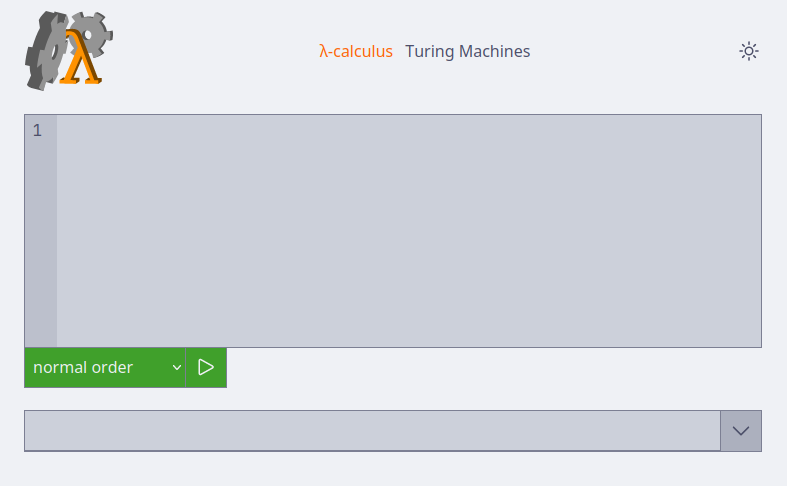
\includegraphics[width=10cm]{empty.png}
  \caption{The λ-calculus page}
  \label{fig:lam_empty}
\end{figure}

\Cref{fig:lam_filled} shows the text editor filled with a λ-calculus term that,
when reduced, results in the Church numeral for \(2 + 1\), i.e. the successor of
\(2\).

\begin{figure}[h]
  \centering
  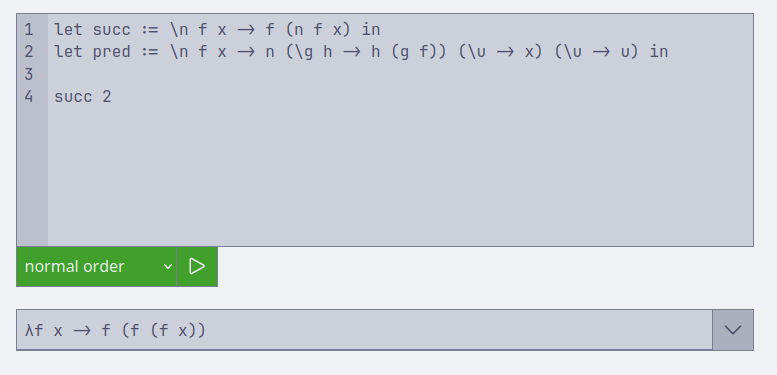
\includegraphics[width=12cm]{filled.png}
  \caption{An example term to reduce}
  \label{fig:lam_filled}
\end{figure}

In particular, this example displays some extra, purely syntactic,
conveniences over our textbook definition of the λ-calculus given earlier:
\begin{enumerate}
  \item
    Abstractions are written as \verb|\x -> t| and may bind multiple variables
    at once. Thus, an abstraction that binds two variables may be written
    \verb|\x y -> t|, which is parsed as being equivalent to the nested
    abstractions \(\labs*{x}{\labs*{y}{t}}\).
  \item
    The syntactic notion of a \emph{let expression} is implemented as a
    shorthand for referencing the same λ-term in multiple places. Importantly,
    the let expression \verb|let f := s in t| is parsed as being equivalent to a
    term of the form \(\lapp*{\labs*{f}{t}}{s}\), and consequently, does not add
    any extra power to the λ-calculus. That is, there is no way to refer to the
    name \(f\) \emph{within} the term \(t\), as would be allowed by recursive
    let bindings in functional programming languages.
  \item
    Natural numbers are interpreted by the parser as a shorthand for their
    corresponding Church numerals. Hence, \(0\) is recognised as
    \(\labs*{f}{\labs*{x}{x}}\), \(1\) as
    \(\labs*{f}{\labs*{x}{\lapp*{f}{x}}}\), \(2\) as
    \(\labs*{f}{\labs*{x}{\lapp*{f}{\lapp*{f}{x}}}}\), and so on.
\end{enumerate}

To reduce the currently entered term, simply press the green \enquote{play}
button. If you wish to view each reduction step individually, you may press the
down arrow next to the output tray to do so, as seen in \Cref{fig:lam_expanded}.

\begin{figure}
  \centering
  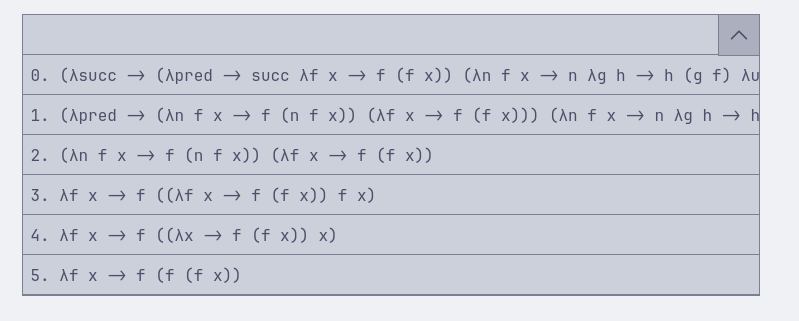
\includegraphics[width=12cm]{expanded.png}
  \caption{The expanded output tray}
  \label{fig:lam_expanded}
\end{figure}

\printbibliography[heading=bibintoc]

\end{document}
